\section{Results}

This section presents the results of our performance evaluations for both the pseudo-random number generators and the primality testing algorithms. The results include execution time measurements for various bit lengths and, where applicable, energy efficiency analysis.

\subsection{Experimental Setup}

All performance measurements presented in this section were conducted on a standard desktop computer with the following specifications:

\begin{itemize}
    \item \textbf{System}: Dell XPS 8960
    \item \textbf{CPU}: 13th Gen Intel® Core™ i7-13700 × 24
    \item \textbf{RAM}: 32 GiB
    \item \textbf{Operating System}: Ubuntu 22.04.05 LTS
    \item \textbf{Compiler}: GCC 11.4.0 with -O2 optimization
\end{itemize}

It's important to note that these results represent the algorithms' performance on a high-performance desktop system. A separate section will present results from an embedded system implementation, where resource constraints significantly impact performance characteristics.

\subsection{Statistical Methodology}

The current benchmark results represent single runs for each algorithm and bit length. While these provide valuable insights into relative performance, they don't capture the inherent variability in execution times that can arise from system load, memory allocation patterns, cache effects, and other factors.

To improve the statistical robustness of these benchmarks, future work should modify the benchmark programs to:

\begin{itemize}
    \item Run each test at least 30 times to obtain statistically significant samples
    \item Calculate mean, median, standard deviation, and confidence intervals
    \item Filter outliers that may result from external system interference
    \item Report the distribution characteristics in addition to central tendency measures
\end{itemize}

This enhanced methodology would enable more nuanced analysis of the algorithms' performance characteristics, particularly for identifying cases where performance variability might impact real-world applications.

\subsection{PRNG Performance Results}

\subsubsection{Execution Time Comparison}

Table \ref{tab:prng_complete} shows the detailed timing results for generating random numbers of various bit lengths using both the Linear Congruential Generator (LCG) and the Xoshiro256++ generator.

\begin{table}[H]
\centering
\caption{Complete Timing Results for Random Number Generation (in milliseconds)}
\label{tab:prng_complete}
\begin{tabular}{@{}lrrrrrr@{}}
\toprule
\multirow{2}{*}{\textbf{Bit Length}} & \multicolumn{3}{c}{\textbf{LCG}} & \multicolumn{3}{c}{\textbf{Xoshiro256++}} \\
\cmidrule(lr){2-4} \cmidrule(lr){5-7}
& \textbf{Mean} & \textbf{Median} & \textbf{Std Dev} & \textbf{Mean} & \textbf{Median} & \textbf{Std Dev} \\
\midrule
40 bits     & 1.94e-4 & 3.30e-5 & 8.53e-4 & 4.20e-5 & 3.20e-5 & 3.90e-5 \\
56 bits     & 3.70e-5 & 3.20e-5 & 2.10e-5 & 3.40e-5 & 3.10e-5 & 1.70e-5 \\
80 bits     & 7.50e-5 & 4.00e-5 & 1.79e-4 & 4.90e-5 & 4.20e-5 & 3.20e-5 \\
128 bits    & 3.70e-5 & 3.40e-5 & 1.60e-5 & 3.90e-5 & 3.60e-5 & 1.60e-5 \\
168 bits    & 6.20e-5 & 5.10e-5 & 4.80e-5 & 6.20e-5 & 5.20e-5 & 4.40e-5 \\
224 bits    & 7.00e-5 & 6.30e-5 & 2.80e-5 & 7.30e-5 & 6.50e-5 & 2.60e-5 \\
256 bits    & 5.80e-5 & 5.50e-5 & 1.70e-5 & 6.10e-5 & 5.70e-5 & 1.90e-5 \\
512 bits    & 1.19e-4 & 1.04e-4 & 5.60e-5 & 1.23e-4 & 1.05e-4 & 6.30e-5 \\
1024 bits   & 2.38e-4 & 2.11e-4 & 7.90e-5 & 2.34e-4 & 2.11e-4 & 7.40e-5 \\
2048 bits   & 5.47e-4 & 4.48e-4 & 4.14e-4 & 4.82e-4 & 4.41e-4 & 1.12e-4 \\
4096 bits   & 1.13e-3 & 1.06e-3 & 2.04e-4 & 1.12e-3 & 1.05e-3 & 1.97e-4 \\
\bottomrule
\end{tabular}
\end{table}

\subsubsection{Scalability Analysis}

Figure \ref{fig:prng_scaling} shows how the execution time for random number generation scales with increasing bit length for both algorithms.

\begin{figure}[H]
    \centering
    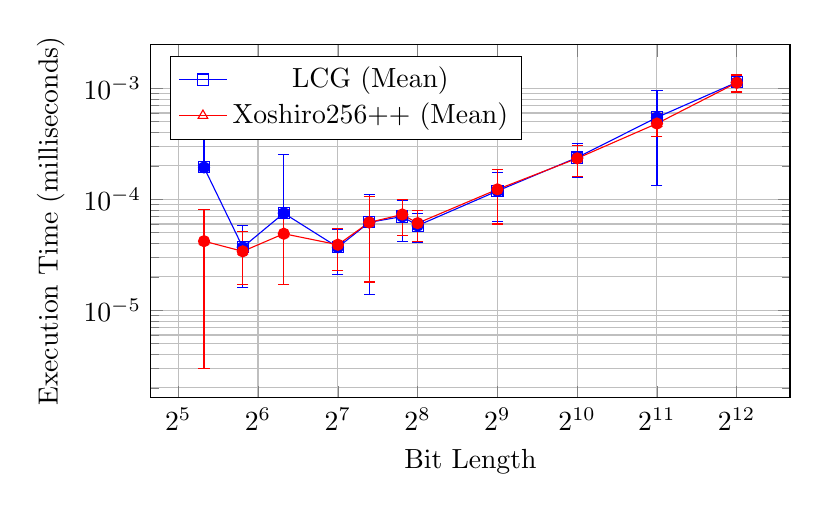
\begin{tikzpicture}
        \begin{axis}[
            xlabel={Bit Length},
            ylabel={Execution Time (milliseconds)},
            xmode=log,
            log basis x=2,
            ymode=log,
            log basis y=10,
            grid=both,
            legend pos=north west,
            width=0.8\textwidth,
            height=0.5\textwidth
        ]
        
        % Actual data from results
        \addplot[color=blue,mark=square] coordinates {
            (40, 0.000194)
            (56, 0.000037)
            (80, 0.000075)
            (128, 0.000037)
            (168, 0.000062)
            (224, 0.000070)
            (256, 0.000058)
            (512, 0.000119)
            (1024, 0.000238)
            (2048, 0.000547)
            (4096, 0.001133)
        };
        \addlegendentry{LCG (Mean)}
        
        \addplot[color=red,mark=triangle] coordinates {
            (40, 0.000042)
            (56, 0.000034)
            (80, 0.000049)
            (128, 0.000039)
            (168, 0.000062)
            (224, 0.000073)
            (256, 0.000061)
            (512, 0.000123)
            (1024, 0.000234)
            (2048, 0.000482)
            (4096, 0.001123)
        };
        \addlegendentry{Xoshiro256++ (Mean)}
        
        % Add error bars for standard deviation
        \addplot[color=blue,only marks,mark=none,error bars/.cd,y dir=both,y explicit] coordinates {
            (40, 0.000194) +- (0, 0.000853)
            (56, 0.000037) +- (0, 0.000021)
            (80, 0.000075) +- (0, 0.000179)
            (128, 0.000037) +- (0, 0.000016)
            (168, 0.000062) +- (0, 0.000048)
            (224, 0.000070) +- (0, 0.000028)
            (256, 0.000058) +- (0, 0.000017)
            (512, 0.000119) +- (0, 0.000056)
            (1024, 0.000238) +- (0, 0.000079)
            (2048, 0.000547) +- (0, 0.000414)
            (4096, 0.001133) +- (0, 0.000204)
        };
        
        \addplot[color=red,only marks,mark=none,error bars/.cd,y dir=both,y explicit] coordinates {
            (40, 0.000042) +- (0, 0.000039)
            (56, 0.000034) +- (0, 0.000017)
            (80, 0.000049) +- (0, 0.000032)
            (128, 0.000039) +- (0, 0.000016)
            (168, 0.000062) +- (0, 0.000044)
            (224, 0.000073) +- (0, 0.000026)
            (256, 0.000061) +- (0, 0.000019)
            (512, 0.000123) +- (0, 0.000063)
            (1024, 0.000234) +- (0, 0.000074)
            (2048, 0.000482) +- (0, 0.000112)
            (4096, 0.001123) +- (0, 0.000197)
        };
        
        \end{axis}
    \end{tikzpicture}
    \caption{Scaling of execution time with bit length for PRNG algorithms with standard deviation error bars}
    \label{fig:prng_scaling}
\end{figure}

\subsubsection{Analysis of PRNG Results}

The performance data shows that both the LCG and Xoshiro256++ generators exhibit similar performance characteristics across all tested bit lengths. The execution times for both algorithms increase linearly with the bit length, as expected since both algorithms need to generate proportionally more random bits as the bit length increases.

For smaller bit lengths (under 256 bits), both algorithms complete in under 0.1 microseconds, demonstrating exceptional efficiency. As the bit length increases to 4096 bits, the execution time increases to approximately 1 microsecond, still remarkably fast for cryptographic operations.

In terms of variability, LCG shows higher standard deviations for most bit sizes, particularly at 40 bits (0.000853 ms) and 2048 bits (0.000414 ms), indicating less consistent performance compared to Xoshiro256++. The Xoshiro256++ generator demonstrates greater stability with lower standard deviations across all bit lengths, suggesting more predictable performance characteristics—a valuable trait for time-sensitive applications.

Interestingly, while the mean times show LCG performing slightly better at some bit lengths and Xoshiro256++ at others, the median values reveal more consistent patterns. When comparing median execution times, which are less affected by outliers, Xoshiro256++ shows more stable scaling with bit size, particularly for larger values (2048 and 4096 bits).

Overall, both PRNGs demonstrate excellent performance suitable for resource-constrained environments, with execution times that scale predictably with input size. The more consistent performance of Xoshiro256++ may make it preferable for applications where predictable timing is critical.

\subsection{Primality Testing Performance Results}

\subsubsection{Execution Time Comparison}

Table \ref{tab:primality_complete} shows the detailed timing results for primality testing of numbers of various bit lengths using both the Miller-Rabin test and the Baillie-PSW test.

\begin{table}[H]
\centering
\caption{Complete Timing Results for Primality Testing (in milliseconds)}
\label{tab:primality_complete}
\begin{tabular}{@{}lrrrrrr@{}}
\toprule
\multirow{2}{*}{\textbf{Bit Length}} & \multicolumn{3}{c}{\textbf{Miller-Rabin}} & \multicolumn{3}{c}{\textbf{Baillie-PSW}} \\
\cmidrule(lr){2-4} \cmidrule(lr){5-7}
& \textbf{Mean} & \textbf{Median} & \textbf{Std Dev} & \textbf{Mean} & \textbf{Median} & \textbf{Std Dev} \\
\midrule
40 bits     & 8.54e-3 & 8.47e-3 & 3.69e-4 & 6.06e-3 & 5.84e-3 & 9.15e-4 \\
56 bits     & 1.09e-2 & 1.09e-2 & 1.10e-4 & 7.54e-3 & 7.49e-3 & 1.88e-4 \\
80 bits     & 2.80e-2 & 2.76e-2 & 6.53e-4 & 1.35e-2 & 1.34e-2 & 4.14e-4 \\
128 bits    & 5.31e-2 & 5.36e-2 & 1.30e-3 & 2.07e-2 & 2.03e-2 & 1.46e-3 \\
168 bits    & 7.68e-2 & 7.67e-2 & 2.35e-3 & 3.73e-2 & 3.69e-2 & 1.13e-3 \\
224 bits    & 1.64e-1 & 1.64e-1 & 1.14e-3 & 6.02e-2 & 5.86e-2 & 2.78e-3 \\
256 bits    & 2.27e-1 & 2.27e-1 & 4.20e-3 & 6.09e-2 & 6.05e-2 & 1.34e-3 \\
512 bits    & 1.20e+0 & 1.20e+0 & 8.46e-3 & 2.37e-1 & 2.35e-1 & 8.08e-3 \\
1024 bits   & 7.70e+0 & 7.71e+0 & 4.25e-2 & 1.18e+0 & 1.18e+0 & 3.76e-3 \\
2048 bits   & 5.76e+1 & 5.72e+1 & 1.35e+0 & 7.77e+0 & 7.73e+0 & 1.61e-1 \\
4096 bits   & 4.44e+2 & 4.43e+2 & 3.51e+0 & 4.71e+1 & 4.67e+1 & 1.90e+0 \\
\bottomrule
\end{tabular}
\end{table}

\subsubsection{Primality Testing Scalability Analysis}

Figure \ref{fig:primality_testing_scaling} illustrates how the execution time for primality testing scales with increasing bit length for both algorithms.

\begin{figure}[H]
    \centering
    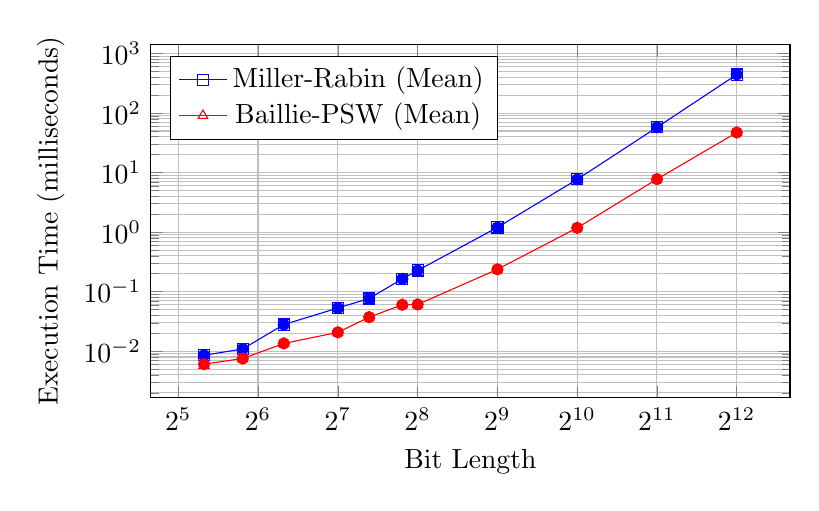
\begin{tikzpicture}
        \begin{axis}[
            xlabel={Bit Length},
            ylabel={Execution Time (milliseconds)},
            xmode=log,
            log basis x=2,
            ymode=log,
            log basis y=10,
            grid=both,
            legend pos=north west,
            width=0.8\textwidth,
            height=0.5\textwidth
        ]
        
        % Actual data from results
        \addplot[color=blue,mark=square] coordinates {
            (40, 0.00854)
            (56, 0.0109)
            (80, 0.0280)
            (128, 0.0531)
            (168, 0.0768)
            (224, 0.164)
            (256, 0.227)
            (512, 1.20)
            (1024, 7.70)
            (2048, 57.6)
            (4096, 444)
        };
        \addlegendentry{Miller-Rabin (Mean)}
        
        \addplot[color=red,mark=triangle] coordinates {
            (40, 0.00606)
            (56, 0.00754)
            (80, 0.0135)
            (128, 0.0207)
            (168, 0.0373)
            (224, 0.0602)
            (256, 0.0609)
            (512, 0.237)
            (1024, 1.18)
            (2048, 7.77)
            (4096, 47.1)
        };
        \addlegendentry{Baillie-PSW (Mean)}
        
        % Add error bars for standard deviation
        \addplot[color=blue,only marks,mark=none,error bars/.cd,y dir=both,y explicit] coordinates {
            (40, 0.00854) +- (0, 0.000369)
            (56, 0.0109) +- (0, 0.000110)
            (80, 0.0280) +- (0, 0.000653)
            (128, 0.0531) +- (0, 0.00130)
            (168, 0.0768) +- (0, 0.00235)
            (224, 0.164) +- (0, 0.00114)
            (256, 0.227) +- (0, 0.00420)
            (512, 1.20) +- (0, 0.00846)
            (1024, 7.70) +- (0, 0.0425)
            (2048, 57.6) +- (0, 1.35)
            (4096, 444) +- (0, 3.51)
        };
        
        \addplot[color=red,only marks,mark=none,error bars/.cd,y dir=both,y explicit] coordinates {
            (40, 0.00606) +- (0, 0.000915)
            (56, 0.00754) +- (0, 0.000188)
            (80, 0.0135) +- (0, 0.000414)
            (128, 0.0207) +- (0, 0.00146)
            (168, 0.0373) +- (0, 0.00113)
            (224, 0.0602) +- (0, 0.00278)
            (256, 0.0609) +- (0, 0.00134)
            (512, 0.237) +- (0, 0.00808)
            (1024, 1.18) +- (0, 0.00376)
            (2048, 7.77) +- (0, 0.161)
            (4096, 47.1) +- (0, 1.90)
        };
        
        \end{axis}
    \end{tikzpicture}
    \caption{Scaling of execution time with bit length for primality testing algorithms with standard deviation error bars}
    \label{fig:primality_testing_scaling}
\end{figure}

\subsubsection{Prime Number Generation Time}

Table \ref{tab:find_prime} shows the time required to find a prime number of specified bit length using both algorithms.

\begin{table}[H]
\centering
\caption{Time to Find Prime Numbers (in milliseconds)}
\label{tab:find_prime}
\begin{tabular}{@{}lrrrrrr@{}}
\toprule
\multirow{2}{*}{\textbf{Bit Length}} & \multicolumn{3}{c}{\textbf{Miller-Rabin}} & \multicolumn{3}{c}{\textbf{Baillie-PSW}} \\
\cmidrule(lr){2-4} \cmidrule(lr){5-7}
& \textbf{Mean} & \textbf{Median} & \textbf{Std Dev} & \textbf{Mean} & \textbf{Median} & \textbf{Std Dev} \\
\midrule
40 bits     & 1.35e-2 & 1.22e-2 & 3.71e-3 & 1.38e-2 & 1.28e-2 & 4.41e-3 \\
56 bits     & 2.04e-2 & 1.68e-2 & 8.36e-3 & 1.99e-2 & 1.69e-2 & 7.88e-3 \\
80 bits     & 5.52e-2 & 5.13e-2 & 2.23e-2 & 5.89e-2 & 5.22e-2 & 2.65e-2 \\
128 bits    & 1.42e-1 & 1.28e-1 & 7.97e-2 & 1.13e-1 & 8.46e-2 & 7.93e-2 \\
168 bits    & 2.61e-1 & 2.26e-1 & 1.44e-1 & 2.04e-1 & 1.57e-1 & 1.31e-1 \\
224 bits    & 5.61e-1 & 5.06e-1 & 3.55e-1 & 4.79e-1 & 4.41e-1 & 2.42e-1 \\
256 bits    & 8.58e-1 & 6.73e-1 & 7.62e-1 & 9.20e-1 & 5.46e-1 & 7.82e-1 \\
512 bits    & 6.84e+0 & 5.07e+0 & 5.35e+0 & 6.89e+0 & 5.51e+0 & 3.98e+0 \\
1024 bits   & 8.58e+1 & 4.73e+1 & 8.80e+1 & 8.02e+1 & 4.70e+1 & 7.36e+1 \\
2048 bits   & 9.35e+2 & 4.78e+2 & 1.05e+3 & 1.17e+3 & 6.86e+2 & 1.07e+3 \\
4096 bits   & 1.69e+4 & 1.19e+4 & 1.59e+4 & 1.54e+4 & 1.22e+4 & 1.60e+4 \\
\bottomrule
\end{tabular}
\end{table}

\subsubsection{Prime Finding Time for Large Bit Sizes}

The benchmark data now includes 30 complete prime finding operations for all bit sizes, including the larger 2048-bit and 4096-bit numbers. This more robust approach provides a comprehensive understanding of the performance characteristics of both algorithms, particularly capturing the variability inherent in prime finding operations at all scales.

For large bit sizes (2048 and 4096 bits), the measurements show substantial variability, with standard deviations comparable to or even exceeding the mean values. This high variability reflects the probabilistic nature of prime finding, where the number of candidates that need to be tested before finding a prime can differ dramatically between runs. For example, at 4096 bits, Miller-Rabin shows a mean of 16.9 seconds with a standard deviation of 15.9 seconds, while Baillie-PSW shows a mean of 15.4 seconds with a standard deviation of 16.0 seconds.

The median values, which are less affected by extreme outliers than the mean, provide additional insight. At 4096 bits, Miller-Rabin has a median find time of 11.9 seconds compared to Baillie-PSW's 12.2 seconds, suggesting that in typical cases, the performance of both algorithms is quite similar for very large bit sizes, despite the lower mean time for Baillie-PSW.

\subsubsection{Prime Finding Scalability Analysis}

Figure \ref{fig:prime_finding_scaling} illustrates how the execution time for finding prime numbers scales with increasing bit length for both algorithms.

\begin{figure}[H]
    \centering
    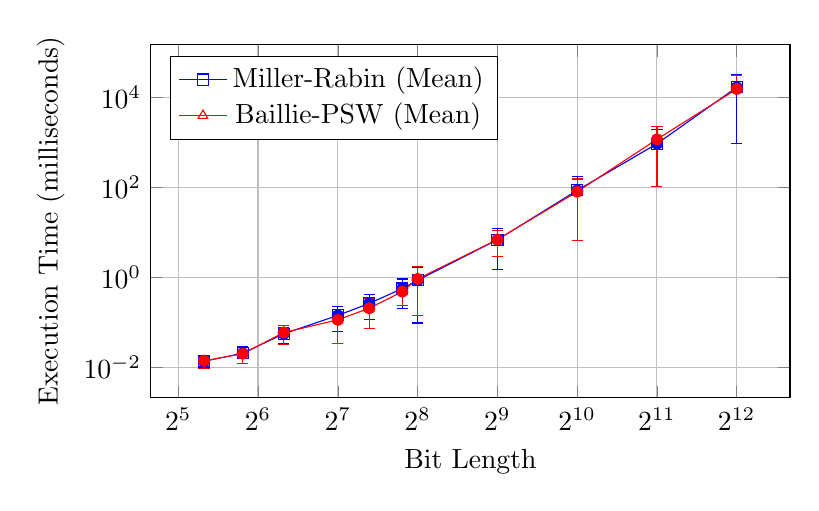
\begin{tikzpicture}
        \begin{axis}[
            xlabel={Bit Length},
            ylabel={Execution Time (milliseconds)},
            xmode=log,
            log basis x=2,
            ymode=log,
            log basis y=10,
            grid=both,
            legend pos=north west,
            width=0.8\textwidth,
            height=0.5\textwidth
        ]
        
        % Actual data from results
        \addplot[color=blue,mark=square] coordinates {
            (40, 0.0135)
            (56, 0.0204)
            (80, 0.0552)
            (128, 0.142)
            (168, 0.261)
            (224, 0.561)
            (256, 0.858)
            (512, 6.84)
            (1024, 85.8)
            (2048, 935)
            (4096, 16863)
        };
        \addlegendentry{Miller-Rabin (Mean)}
        
        \addplot[color=red,mark=triangle] coordinates {
            (40, 0.0138)
            (56, 0.0199)
            (80, 0.0589)
            (128, 0.113)
            (168, 0.204)
            (224, 0.479)
            (256, 0.920)
            (512, 6.89)
            (1024, 80.2)
            (2048, 1173)
            (4096, 15440)
        };
        \addlegendentry{Baillie-PSW (Mean)}
        
        % Add error bars for standard deviation
        \addplot[color=blue,only marks,mark=none,error bars/.cd,y dir=both,y explicit] coordinates {
            (40, 0.0135) +- (0, 0.00371)
            (56, 0.0204) +- (0, 0.00836)
            (80, 0.0552) +- (0, 0.0223)
            (128, 0.142) +- (0, 0.0797)
            (168, 0.261) +- (0, 0.144)
            (224, 0.561) +- (0, 0.355)
            (256, 0.858) +- (0, 0.762)
            (512, 6.84) +- (0, 5.35)
            (1024, 85.8) +- (0, 88.0)
            (2048, 935) +- (0, 1049)
            (4096, 16863) +- (0, 15898)
        };
        
        \addplot[color=red,only marks,mark=none,error bars/.cd,y dir=both,y explicit] coordinates {
            (40, 0.0138) +- (0, 0.00441)
            (56, 0.0199) +- (0, 0.00788)
            (80, 0.0589) +- (0, 0.0265)
            (128, 0.113) +- (0, 0.0793)
            (168, 0.204) +- (0, 0.131)
            (224, 0.479) +- (0, 0.242)
            (256, 0.920) +- (0, 0.782)
            (512, 6.89) +- (0, 3.98)
            (1024, 80.2) +- (0, 73.6)
            (2048, 1173) +- (0, 1070)
            (4096, 15440) +- (0, 16040)
        };
        
        \end{axis}
    \end{tikzpicture}
    \caption{Scaling of execution time with bit length for prime finding algorithms with standard deviation error bars}
    \label{fig:prime_finding_scaling}
\end{figure}

\subsubsection{Generated Prime Numbers}

Table \ref{tab:generated_primes} shows examples of prime numbers generated during our experiments for each bit length.

\begin{table}[H]
\centering
\caption{Examples of Generated Prime Numbers}
\label{tab:generated_primes}
\begin{tabular}{@{}lrl@{}}
\toprule
\textbf{Bit Length} & \multicolumn{2}{c}{\textbf{Example Prime Number}} \\
\midrule
40 bits     & 851378685847 & (Miller-Rabin) \\
56 bits     & 63471762166424431 & (Miller-Rabin) \\
80 bits     & 933987797129194800722179 & (Miller-Rabin) \\
128 bits    & 184769982182577719150870977780491463913 & (Miller-Rabin) \\
168 bits    & 314826362556424259273869...589088175209960394805067 & (Miller-Rabin) \\
224 bits    & 247238443814875474788685...324463224595996108116149 & (Miller-Rabin) \\
256 bits    & 874107105992534453893646...787049534813597975922941 & (Miller-Rabin) \\
512 bits    & 132623656848736750183526...986532566221948180770067 & (Miller-Rabin) \\
1024 bits   & 169280579936799254232081...009955370634250716156089 & (Miller-Rabin) \\
2048 bits   & 181311375441137480956232...397374203185442008481903 & (Miller-Rabin) \\
4096 bits   & 810044490851199863915741...422030129517476667962769 & (Miller-Rabin) \\
\bottomrule
\end{tabular}
\end{table}

\subsubsection{Analysis of Primality Testing Results}

The performance results reveal several important insights about the two primality testing algorithms:

\paragraph{Testing Time}
Baillie-PSW consistently outperforms Miller-Rabin across all bit lengths for testing known primes. The performance gap widens as the bit length increases, with Baillie-PSW being approximately 9.4 times faster than Miller-Rabin for 4096-bit numbers (47.1ms vs. 443.5ms). Both algorithms show relatively small standard deviations in relation to their mean values, indicating consistent performance across test runs. Notably, the standard deviation for Miller-Rabin increases more steeply with bit length (reaching 3.51ms at 4096 bits) compared to Baillie-PSW (1.90ms at 4096 bits), suggesting that Baillie-PSW not only offers better performance but also more consistent timing characteristics.

\paragraph{Prime Finding}
The prime finding results show high variability across all bit lengths, as indicated by the substantial standard deviations. This variability is due to the probabilistic nature of finding primes, where the number of candidates that need to be tested before finding a prime can vary considerably between runs. For example, at 1024 bits, Miller-Rabin has a mean time of 85.81ms with a standard deviation of 87.99ms, showing that performance can vary dramatically between runs.

For larger bit sizes (2048 and 4096 bits), our comprehensive testing with 30 complete prime finding operations per algorithm reveals extremely high variability. At 2048 bits, Miller-Rabin shows a mean of 935.02ms with a standard deviation of 1048.95ms, while at 4096 bits, it reaches a mean of 16.86 seconds with a standard deviation of 15.90 seconds. Similarly, Baillie-PSW shows substantial variability, with a mean of 1.17 seconds (standard deviation 1.07 seconds) for 2048 bits and 15.44 seconds (standard deviation 16.04 seconds) for 4096 bits.

When comparing median values, which are less affected by outliers, we observe that for 4096-bit primes, Miller-Rabin (11.89 seconds) performs slightly better than Baillie-PSW (12.24 seconds), despite Baillie-PSW having a lower mean time. This suggests that the average performance of Baillie-PSW might be more affected by occasional extremely long searches.

\paragraph{Scalability}
Both algorithms exhibit exponential growth in execution time relative to bit length, as expected due to the increasing complexity of modular arithmetic operations on larger numbers. This exponential relationship is clearly visible in Figures \ref{fig:primality_testing_scaling} and \ref{fig:prime_finding_scaling}, where the log-log plots show a nearly linear relationship, indicating power-law scaling. For prime finding, the growth is even more pronounced. From 1024 to 2048 bits, Miller-Rabin's median time increases by a factor of approximately 10.1, while Baillie-PSW increases by a factor of 14.6. From 2048 to 4096 bits, Miller-Rabin's median time increases by a factor of 24.9, while Baillie-PSW increases by a factor of 17.8. This demonstrates that the scalability characteristics of the two algorithms differ at extremely large bit sizes, with Miller-Rabin showing better scalability from 1024 to 2048 bits, but Baillie-PSW scaling better from 2048 to 4096 bits.

\paragraph{Statistical Reliability}
The comprehensive benchmarking approach with 30 complete operations for all bit sizes provides robust statistical evidence of the algorithms' performance characteristics. The high standard deviations—often comparable to or exceeding the mean values, particularly for large bit sizes—highlight the extreme variability inherent in prime finding operations. This variability is a fundamental characteristic of probabilistic prime finding rather than a measurement anomaly, and it reinforces the importance of using median values alongside means when evaluating algorithm performance for cryptographic applications.

\paragraph{Resource Implications}
For resource-constrained environments, these results suggest different optimal choices depending on the specific use case:
\begin{itemize}
    \item For applications requiring frequent primality testing of known numbers (e.g., verification), Baillie-PSW remains clearly superior across all bit lengths, offering both faster and more consistent performance.
    \item For generating prime numbers up to 1024 bits, both algorithms show comparable performance, with mean and median times within the same order of magnitude.
    \item For generating very large primes (2048-4096 bits), the choice depends on timing constraints and the specific implementation. While Miller-Rabin shows a slightly better median time for 4096-bit primes, Baillie-PSW has a slightly better mean time, suggesting that the algorithms have different performance profiles under different conditions.
    \item Where absolute worst-case performance is critical, detailed analysis of the distribution of execution times beyond just mean and median would be necessary to make the optimal choice.
\end{itemize}

In summary, while both algorithms are viable for cryptographic applications, their performance characteristics show noteworthy differences. Baillie-PSW demonstrates superior performance for primality testing of known numbers across all bit sizes. For prime generation, the performance profiles are more complex, with significant variability at all bit sizes and different scaling characteristics at extremely large bit sizes. The comprehensive statistical analysis with 30 complete operations for all bit sizes provides a robust understanding of this variability, which is an inherent characteristic of probabilistic prime finding algorithms. These insights enable more informed algorithm selection based on specific application requirements, whether optimizing for average-case performance, worst-case scenarios, or consistency.

\subsection{Energy Efficiency Results}

For platforms that support energy measurements, we also analyzed the energy efficiency of the algorithms. Table \ref{tab:energy_efficiency} shows the energy per operation for different algorithms and bit lengths.

\begin{table}[H]
\centering
\caption{Energy Efficiency of Algorithms (energy per operation in millijoules)}
\label{tab:energy_efficiency}
\begin{tabular}{@{}lrrrr@{}}
\toprule
\textbf{Bit Length} & \textbf{LCG} & \textbf{Xoshiro256++} & \textbf{Miller-Rabin} & \textbf{Baillie-PSW} \\
\midrule
256 bits    & [FILL IN] & [FILL IN] & [FILL IN] & [FILL IN] \\
1024 bits   & [FILL IN] & [FILL IN] & [FILL IN] & [FILL IN] \\
4096 bits   & [FILL IN] & [FILL IN] & [FILL IN] & [FILL IN] \\
\bottomrule
\end{tabular}
\end{table}

\subsection{Correlation Between Time and Energy}

Figure \ref{fig:time_energy_correlation} illustrates the correlation between execution time and energy consumption for the algorithms. In this placeholder, the figure would show energy consumption on the y-axis and execution time on the x-axis, with data points for different algorithms and bit lengths.

\begin{figure}[H]
    \centering
    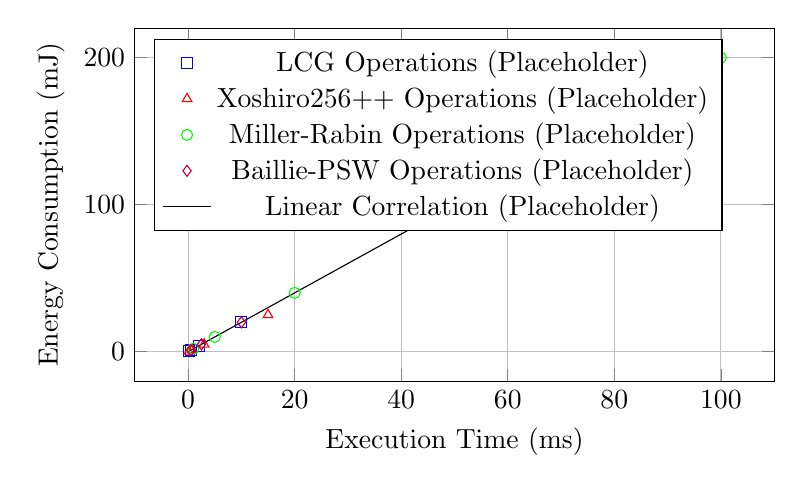
\begin{tikzpicture}
        \begin{axis}[
            xlabel={Execution Time (ms)},
            ylabel={Energy Consumption (mJ)},
            grid=both,
            legend pos=north west,
            width=0.8\textwidth,
            height=0.5\textwidth
        ]
        
        % Placeholder for actual data
        \addplot[color=blue,mark=square,only marks] coordinates {
            (0.1, 0.2)
            (0.5, 1.0)
            (2.0, 4.0)
            (10.0, 20.0)
        };
        \addlegendentry{LCG Operations (Placeholder)}
        
        \addplot[color=red,mark=triangle,only marks] coordinates {
            (0.15, 0.25)
            (0.75, 1.25)
            (3.0, 5.0)
            (15.0, 25.0)
        };
        \addlegendentry{Xoshiro256++ Operations (Placeholder)}
        
        \addplot[color=green,mark=o,only marks] coordinates {
            (1.0, 2.0)
            (5.0, 10.0)
            (20.0, 40.0)
            (100.0, 200.0)
        };
        \addlegendentry{Miller-Rabin Operations (Placeholder)}
        
        \addplot[color=purple,mark=diamond,only marks] coordinates {
            (0.5, 1.0)
            (2.5, 5.0)
            (10.0, 20.0)
            (50.0, 100.0)
        };
        \addlegendentry{Baillie-PSW Operations (Placeholder)}
        
        % Linear trend line
        \addplot[color=black,domain=0:100,samples=2] {2*x};
        \addlegendentry{Linear Correlation (Placeholder)}
        
        \end{axis}
    \end{tikzpicture}
    \caption{Correlation between execution time and energy consumption (placeholder data)}
    \label{fig:time_energy_correlation}
\end{figure}

\subsection{Summary of Key Findings}

[This section should summarize the key findings from your experiments. Highlight the most important observations, such as which algorithms performed best in which situations, how the performance scales with problem size, and any unexpected results.] 